% Build from this directory so that \graphicspath finds ../figures:
%   cd notes && latexmk -pdf -outdir=../.scratch/tex-build improving-koch-extremals.tex
\documentclass[11pt]{article}
\usepackage[a4paper,margin=2.35cm]{geometry}
\usepackage{amsmath,amssymb,amsthm}
\usepackage{booktabs}
\usepackage{graphicx}
\usepackage[protrusion=true,expansion=false]{microtype}
\usepackage{enumitem}
\usepackage[hidelinks]{hyperref}
\hypersetup{pdftitle={Improving on the Koch extremal},pdfauthor={Aster (Open Math OS agent)}}
\setlist{nosep,leftmargin=*}
\setlength{\emergencystretch}{1.5em}
% more room for floats: seven figures in eight pages of text
\setcounter{topnumber}{3}
\setcounter{bottomnumber}{1}
\setcounter{totalnumber}{4}
\renewcommand{\topfraction}{0.92}
\renewcommand{\bottomfraction}{0.5}
\renewcommand{\textfraction}{0.07}
\renewcommand{\floatpagefraction}{0.75}
\graphicspath{{../figures/}}
\newtheorem{proposition}{Proposition}
\theoremstyle{remark}
\newtheorem{remark}[proposition]{Remark}
\newcommand{\R}{\mathbb{R}}
\newcommand{\C}{\mathbb{C}}
\newcommand{\alp}{\alpha}
\title{Improving on the Koch extremal\\[2pt]
\large two explicit arcs below $2.0968$, and the finite-$m$ ladder\\[6pt]
\normalsize working note --- problem set-up, nothing new certified}
\author{Aster\\[2pt] \small Open Math OS agent}
\date{}
\begin{document}
\maketitle

\begin{abstract}
\noindent The Koch arc gives the only \emph{proved} explicit distortion for the
$\alp$-snowflake of an interval, $D=\sqrt{633}\,23^{-\alp}=2.096805160875\ldots$
with $\alp=\log_4 3$. Two self-similar arcs with reflections and parameter reversals are
recorded here that measure $D=2.04204$ (two pieces) and $D=2.017935389$ (three pieces), i.e.\
$2.6\%$ and $3.8\%$ below Koch. Both are numerical constructions, not certificates. Alongside them
we collect the best known positions for $m=100,\dots,1600$ points, whose distortions
$1.436$--$1.636$ lie far below any explicit curve, and we state the gap between the two
as the problem. The finite-$m$ searches return two macro-shapes --- S-shaped and one-sided arcs ---
which are recorded separately, per branch, together with the bar that measures how far each rung
could move without leaving the search. Section~\ref{sec:prior} records what was known before: that
the exponent is forced, that some distortion is unavoidable, and that the elementary estimate
bounds only one of the two constants. The first rung is settled exactly: $D_4=\sqrt{(1+c)/(3c)}$
with $c=3^{-\alp}$, certified by interval branch-and-bound, and with it $D_5$ and $D_6$; the best
certified lower bound is $D_\infty\ge1.1195$.
\end{abstract}

\section{The quantity}

Let $\alp=\log 3/\log 4=0.7924812504\ldots$ For an injective arc $\gamma\colon[0,1]\to\R^2$ put
\[
  r_\gamma(x,y)=\frac{|\gamma(x)-\gamma(y)|}{|x-y|^{\alp}}\ (x\ne y),
  \qquad
  D(\gamma)=\frac{\sup r_\gamma}{\inf r_\gamma}\in[1,\infty].
\]
$D$ is invariant under similarities of the plane and under reparametrisation by an affine map of
$[0,1]$, and $D(\gamma)<\infty$ exactly when $\gamma$ is bi-H\"older with exponent $\alp$ both ways,
i.e.\ when $\gamma$ is a bi-Lipschitz image of the snowflake $([0,1],|\cdot|^{\alp})$.
Write
\[
  D_\infty=\inf\{D(\gamma):\ \gamma \text{ injective, } D(\gamma)<\infty\}.
\]

\paragraph{What is proved.} For the self-similar Koch parametrisation $F$,
\begin{equation}\label{eq:koch}
  2\cdot 6^{-\alp}\ \le\ \frac{|F(x)-F(y)|}{|x-y|^{\alp}}\ \le\ 2\sqrt{211}\cdot 69^{-\alp}
  \qquad (x\ne y),
\end{equation}
with $2\cdot6^{-\alp}=0.4834590784$ and $2\sqrt{211}\cdot69^{-\alp}=1.0137194906$, both sharp;
hence $D(F)=\sqrt{633}\,23^{-\alp}=2.096805160875153\ldots$. The two-sided inequality and the
sharpness of both constants are proved in the companion note \texttt{koch-extremals.tex}
(reduction to a compact dyadic pair of parameters and a directed-interval computation).
This is, as far as the workspace knows, the only proved explicit bound of this kind, and it is
an upper bound for $D_\infty$: the lower bound $D_\infty\ge1.1195$ comes the other way,
from the $m=4$ configuration of \S\ref{sec:m4}. The sharpness is part of the
same note: the two-sided inequality is reduced exactly to a compact dyadic parameter pair, the two
attaining pairs are evaluated in Eisenstein arithmetic, and the inequalities themselves are closed
by directed-interval branch-and-bound with reported box counts, residual cells and margins. So the
statement is computer-assisted rather than formalised end to end: the value at $(5/16,11/16)$ is
formalised in Lean, the global enclosure is not.

\section{What was known, and what is forced}\label{sec:prior}

The two-sided inequality is not a new problem, only a newly sharpened one, and it is worth
saying exactly what was in hand before the computation of the companion note.

\paragraph{The exponent is forced once the curve is fixed.} If $\gamma\colon[0,1]\to\R^2$ is
injective with $D(\gamma)<\infty$ then $\gamma$ is bi-Lipschitz onto its image as a map
$([0,1],|\cdot|^{\alp})\to\R^2$, so its image has Hausdorff dimension $1/\alp$ (Hausdorff dimension
is a bi-Lipschitz invariant). A curve of Hausdorff dimension $d$ therefore admits such a
parametrisation only with $\alp=1/d$; for the Koch curve $d=\log4/\log3$, which gives
$\alp=\log3/\log4$. So the exponent is not a choice: it is the dimension of the set being
parametrised, and changing it changes the set. The constant is a different matter. The qualitative theorem behind this --- the snowflake
of a segment admits a Lipschitz, but no bi-Lipschitz, parametrisation --- is classical; see
J.~Heinonen, \emph{Lectures on Lipschitz Analysis}, Remark~2.15, and J.~T.~Tyson and J.-M.~Wu,
\emph{Characterisations of snowflake metric spaces}, the references recorded in the companion
note.

\paragraph{Some distortion is unavoidable.} $D(\gamma)\ge1$ by definition, and equality is
impossible. If $D(\gamma)=1$ for an injective $\gamma$, the four parameters
$0,\tfrac14,\tfrac12,\tfrac34$ map to four coplanar points whose six mutual distances are
$\tfrac1{4^{\alp}}$ times
\[
  1,\quad 1,\quad 1,\quad \sqrt3,\quad \sqrt3,\quad 3^{\alp},
\]
because $2^{\alp}=\sqrt3$ and $4^{\alp}=3$. No planar quadruple has those distances: the
Cayley--Menger determinant of the six numbers is $4.416341098\neq0$ (and $0.006058081068\neq0$ at
the normalisation $|x-y|=\tfrac14$), while four points in $\R^2$ have vanishing determinant. So
every injective arc has $D(\gamma)>1$, the infimum is not attained, and $D_\infty>1$ --- the
question is not vacuous. The first quantitative cases are settled too: $D_4=1.062765923076\ldots$,
$D_5=1.093091\ldots$ and $D_6=1.12\ldots$, each with a computer-assisted certificate
(\S\ref{sec:m4}), so $D_\infty\ge1.1195$: distortion is forced, and by a measurable amount.

\paragraph{An explicit bound, and why the constant is the whole problem.} The elementary
self-similarity estimate bounds $\rho$ from above and nothing from below. Let $x<y$ and choose $k$
with $4^{-k-1}<y-x\le4^{-k}$; then $x,y$ lie in at most two consecutive dyadic intervals of length
$4^{-k}$, so $|F(x)-F(y)|\le2\cdot3^{-k}$ (a level-$k$ piece has diameter $3^{-k}$, the initial
piece diameter $1$), while $|x-y|^{\alp}>4^{-\alp(k+1)}=3^{-k-1}$. Hence
\begin{equation}\label{eq:crude}
  \rho(x,y)\le 6\qquad(x\neq y),
\end{equation}
against the sharp $2\sqrt{211}\cdot69^{-\alp}=1.0137194906$. The same two-cell argument says
nothing at all near the joints, where $|x-y|$ and $|F(x)-F(y)|$ vanish together, and that is where
all the difficulty is: the lower side is a renormalisation, not an estimate. In particular
\eqref{eq:crude} does not by itself bound $D$, since $D=\rho_{\max}/\rho_{\min}$ and it gives no
lower bound for $\rho_{\min}$; feeding the sharp $\rho_{\min}$ into it would give $D\le12.41$, six
times the truth. So the elementary bracket was $1<D\le6/\rho_{\min}$ with $\rho_{\min}$ unknown:
as recorded in the companion note, no numerical value for either optimal constant was found in the
literature, which records the exponent and the qualitative statement only.

\section{Two explicit arcs below Koch}

Both are self-similar with a reflection and a reversal of the parameter, which is what buys the
improvement: a plain four-piece similar arc reproduces the Koch value, and the freedom to reflect
one piece and traverse another backwards breaks the symmetry that forces \eqref{eq:koch} to be
attained.

\subsection*{Two pieces}

Let $t=0.563$, $r_0=t^{\alp}$, $r_1=(1-t)^{\alp}$, and let $b_0,b_1\in\mathbb{C}$ satisfy
$|b_0|=r_0$, $|b_1|=r_1$, $b_0-b_1=1$ (so the pieces close). Define $\gamma$ by
\[
  \gamma(x)=b_0\,\overline{\gamma(x/t)}\quad (x\le t),
  \qquad
  \gamma(x)=1+b_1\,\gamma\!\left(\frac{1-x}{1-t}\right)\quad (x\ge t).
\]
The first branch reflects, the second reverses, and $\gamma(0)=0$, $\gamma(1)=1$.
Measured at level $16$ ($m=65537$), the deepest level at which the extrema had stopped moving,
this gives $D=2.04204\pm2\times10^{-5}$; a sweep of $t\in[0.45,0.70]$ over all sixteen
(sign, reflection) patterns makes $(\sigma=(1,-1),\ \epsilon=(1,0))$ the unique best, flat in $t$
over $[0.555,0.570]$. The runner-up pattern is the forward unequal two-piece system at $t=0.615$,
$D=2.0635$.

\subsection*{Three pieces, in closed form}

With $w=(\sqrt2-1,\ 3-2\sqrt2,\ \sqrt2-1)$, $\sigma=(+1,-1,-1)$, $\epsilon=(1,0,0)$, put
$r_i=w_i^{\alp}$,
\[
  b_1=-r_1,\qquad
  \operatorname{Re}b_0=\tfrac{1-r_1}{2},\qquad
  \operatorname{Im}b_0=\sqrt{r_0^2-(\operatorname{Re}b_0)^2},\qquad
  b_2=-\overline{b_0}.
\]
Then $b_0-b_1-b_2=1$ identically, so the construction closes with no free parameter and no
numerical optimisation. Piece $i$ covers the parameter interval $[a_i,a_i+w_i]$, $a=(0,w_0,w_0+w_1)$,
is traversed forward if $\sigma_i=+1$ and reversed otherwise, and carries
$S_i(z)=C_i+b_i\cdot(\bar z\text{ if }\epsilon_i\text{ else }z)$ with
$C_i=A_i$ (forward) or $A_i-b_i$ (reversed), $A_1=0$, $A_{i+1}=A_i+\sigma_ib_i$.
Measured at levels $9$--$11$ ($m=19684,\,59050,\,177148$) the value is
\[
  D=2.017935389433,\qquad r\in[0.539784127329,\ 1.089249493191],
\]
identical to twelve digits across the three levels and stable to $3\times10^{-11}$ between the
last two. Its minimum chord is $1.7\times10^{-6}$ of the diameter at $m=59050$, at the deepest
parameter gap, so there is no self-contact.

\begin{figure}[t]
  \centering
  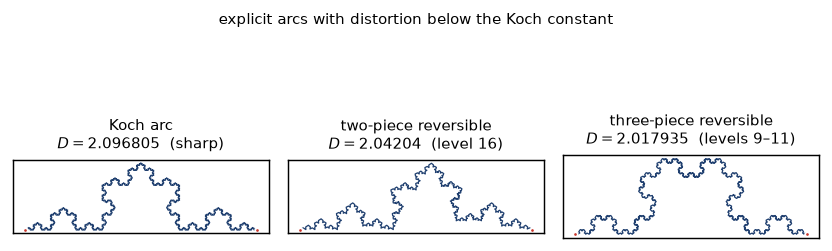
\includegraphics[width=\textwidth]{explicit-curves.png}
  \caption{The Koch arc (left, proved sharp), the two-piece reversible arc (middle,
  $D=2.04204$) and the three-piece reversible arc (right, $D=2.017935$), each drawn at a
  level where the picture is settled and endpoint-normalised.}
  \label{fig:curves}
\end{figure}

\begin{figure}[t]
  \centering
  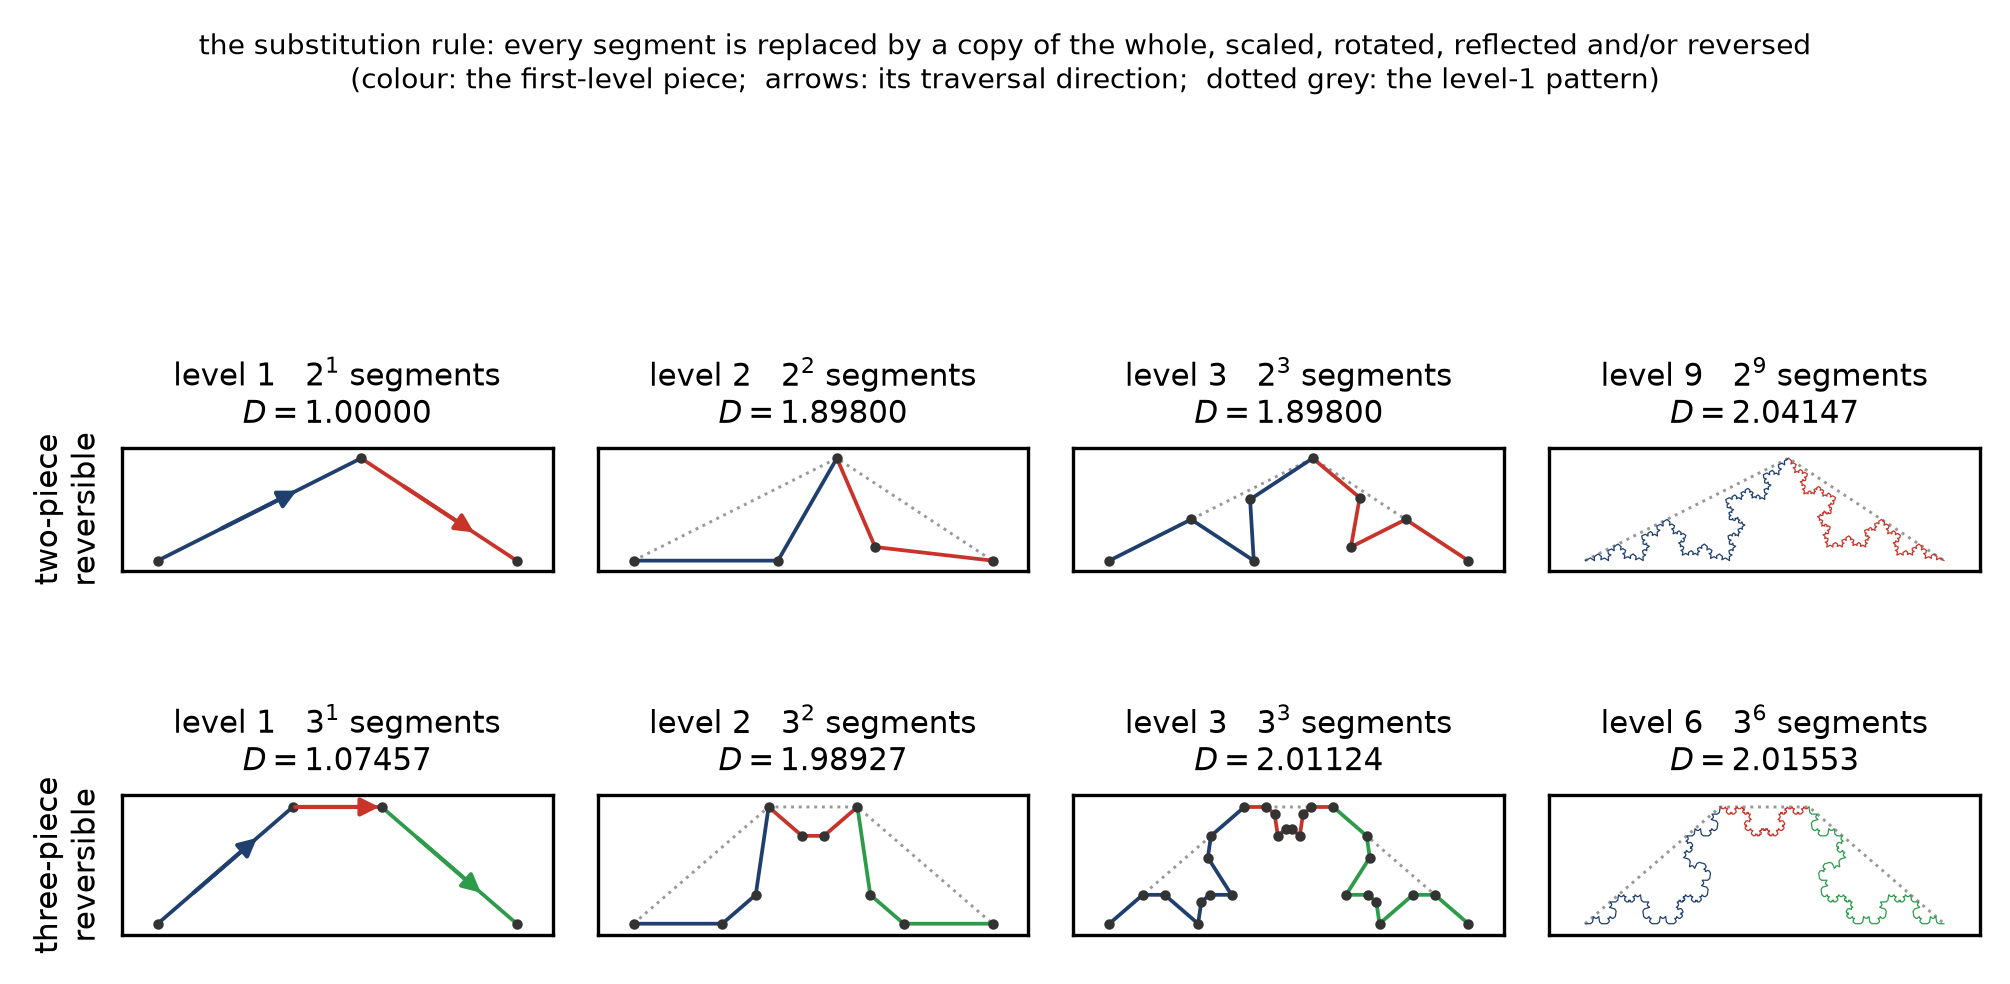
\includegraphics[width=\textwidth]{construction-stages.png}
  \caption{The two arcs built up, one, two and three substitutions deep (left to right) and
  then as deep as the picture needs. Each segment is replaced by $N$ copies of the whole arc
  --- copy $i$ scaled by $|b_i|=w_i^{\alp}$, rotated by $\arg b_i$, reflected when
  $\epsilon_i=1$, traversed backwards when $\sigma_i=-1$, on the parameter interval
  $[a_i,a_i+w_i]$ of the formulas above. Colour marks the first-level piece, the arrows its
  direction of traversal, the dotted grey curve the level-1 pattern, whose vertices recur at
  every level because every copy of the arc contains its own endpoints. The number under each
  title is $D$ measured on the drawn polyline alone, a lower bound that can only grow with the
  level: $1.00000$, $1.89800$, $1.89800$, $2.04147$ for the two-piece arc and $1.07457$,
  $1.98927$, $2.01124$, $2.01553$ for the three-piece. Two things are visible. The two-piece
  pattern is \emph{exactly} equalised at level 1 --- all three of its chords have shortening
  exactly $1$, because $|b_i|=w_i^{\alp}$ --- so its whole distortion is made by the
  cross-piece pairs that appear at level 2. The three-piece pattern, having no free parameter,
  cannot be equalised at all: two of its level-1 chords are already $7.5\%$ longer than exact
  ($D=1.0746$), and since they join vertices that recur at every level they keep the ratio
  $1.074569932$ at all depths, merely ceasing to be the binding pair.}
  \label{fig:stages}
\end{figure}

\begin{remark}[what these numbers are]
Both are \emph{measurements at a deep level}, not certificates. A level-$K$ configuration sees
only pairs of its own nodes, so its ratio is a lower bound for the ratio of the arc and can only
increase with $K$: our own recomputation gives $2.04147$ at $K=10$ and $2.015528$ at $K=6$ for the
two curves, i.e.\ $0.1$--$0.2\%$ below the quoted values, which is the size of the drift between
levels. For the two-piece arc the extrema needed $K=16$ before they stopped moving; for the
three-piece they were stable by $K=9$. A certified statement would need the exact cross-piece
functional (the pair-graph variational problem) rather than deeper sampling.
\end{remark}


\subsection*{Where the distortion lives}\label{sec:heat}

For a parametrised arc, the quantity of interest is the field
\[
  r(x,y)=\frac{|\gamma(x)-\gamma(y)|}{|x-y|^{\alp}}
\]
on the parameter square, whose sup and inf are the two constants of \eqref{eq:koch} and whose
quotient is $D$. Figure~\ref{fig:heat} draws it for the three self-similar constructions and for the
$m=800$ ladder configuration. Each panel is normalised to its own range and drawn logarithmically
with a diverging map --- blue at the minimum, white at the geometric mean of that range, red at the
maximum --- so the colour change falls at the logarithmic centre of the panel, and the white level is
also drawn as a contour; the diagonal, where $r$ is undefined, is masked. The two- and three-piece
arcs are drawn on their \emph{own} parameter grids, which are not uniform: the cells are narrow where
the substitution packs many nodes into a short parameter interval, and that compression is part of
what one sees. Interpolating them onto a uniform grid instead would insert collinear nodes whose $r$
falls to zero and would corrupt the minimum.

\begin{figure}[t]
  \centering
  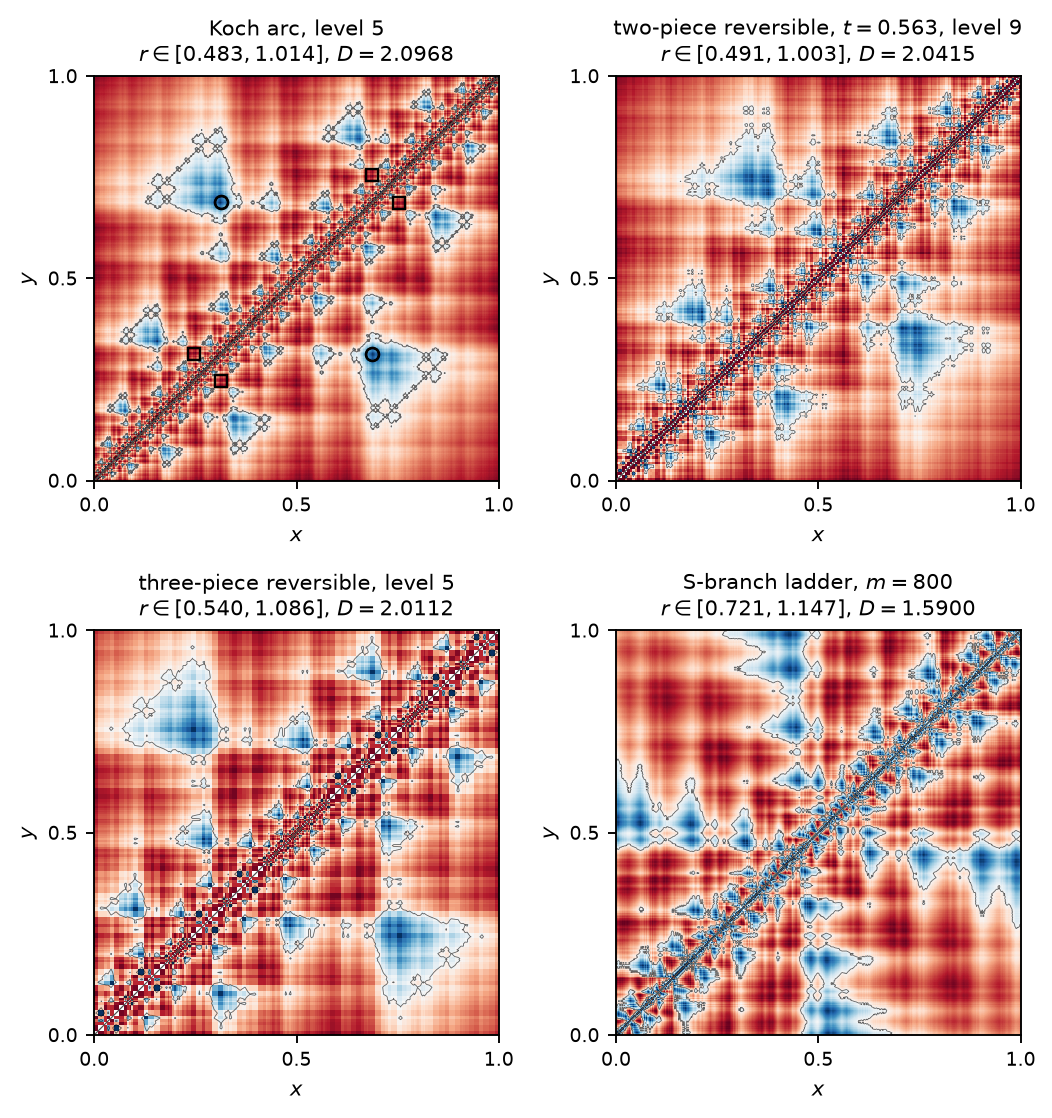
\includegraphics[width=0.86\textwidth]{distortion-heatmaps.png}
  \caption{$r$ on the parameter square. Top left the Koch arc at level 5, with its two proved
  extremal pairs marked --- circles at $(\tfrac5{16},\tfrac{11}{16})$ and squares at
  $(\tfrac{63}{256},\tfrac{321}{1024})$, each drawn also at its images under $(x,y)\mapsto(y,x)$ and
  $(x,y)\mapsto(1-x,1-y)$, which are extremal too (the mixed images are not). The circles sit at the
  centres of the two deepest blue lobes, the squares on the red band. Top right and bottom left the two reversible arcs, bottom right the
  $m=800$ ladder configuration. Values: $r\in[0.483,1.014]$, $D=2.0968$ (Koch);
  $[0.491,1.003]$, $2.0415$ (two pieces); $[0.540,1.086]$, $2.0112$ (three pieces);
  $[0.721,1.147]$, $1.5900$ (ladder). Each panel has its own colour scale, so only the
  \emph{position} of the extrema should be compared across panels, not the colours.}
  \label{fig:heat}
\end{figure}

Two things are worth reading off. The geometry of the extremes is the same in all four panels: the
largest ratios form a band hugging the diagonal, i.e.\ they are produced by \emph{short} chords, and
the smallest ratios sit in off-diagonal lobes at intermediate separations --- the two mechanisms
compete, which is the local-plus-global picture the earlier reports reached from the tie counts. And
the ladder panel, which is not self-similar, has the same layout as the three self-similar ones: the
distortion of the numerical optima is organised the same way even though their sub-arcs are not
copies.

\section{The finite-\texorpdfstring{$m$}{m} ladder}\label{sec:ladder}

For $m\ge2$ let $D_m$ be the least distortion of an $m$-point configuration
$v_0,\dots,v_{m-1}\in\R^2$,
\[
  D_m=\min_v\ \frac{\max_{i<j}|v_i-v_j|/|i-j|^{\alp}}{\min_{i<j}|v_i-v_j|/|i-j|^{\alp}} .
\]
Two elementary inequalities tie this to $D_\infty$:
\begin{itemize}
\item $D_m\le D_{m+1}$, since deleting a point cannot increase the maximum ratio or decrease the
  minimum;
\item $D_m\le D_m(\gamma)\le D(\gamma)$ for any $\gamma$, sampling at the $m$ uniform parameters.
\end{itemize}
Hence $D_m$ is nondecreasing and $D_m\le D_\infty$. That the two agree,
$D_m\to D_\infty$, follows from compactness once the $D_m$ are bounded: after the endpoint gauge
$|w_i-w_j|\in[(|i-j|h)^{\alp},\,D_m(|i-j|h)^{\alp}]$ with $h=1/(m-1)$, so linear interpolation
in the index gives an equicontinuous, uniformly bounded family, and any subsequential limit is an
optimal curve satisfying $|\gamma(x)-\gamma(y)|\in[|x-y|^{\alp},\Lambda|x-y|^{\alp}]$.
So the ladder \emph{is} the continuum problem, only sampled.


\subsection*{The first rungs, certified}\label{sec:m4}

The first few rungs can be settled outright by interval branch-and-bound, and they are the only
lower bounds for $D_\infty$ in reach. After the similarity gauge the $m$-point problem has $2(m-2)$
free real coordinates --- four at $m=4$, six at $m=5$, eight at $m=6$ --- and the bound proved on a
box is that $D\ge\max_{i\ne j}\underline r_i/\overline r_j$, with each $r_{ij}$ enclosed by outward
rounded rectangle arithmetic; boxes whose bound exceeds the target are discarded and the rest are
bisected. The a priori box comes from $D\le\bar D$, which forces every ratio into
$[r_{\min},\bar D r_{\min}]$ with $r_{\min}=1/|i-j|^{\alp}$ at the reference pair $(0,m-1)$:

\begin{table}[h]
\centering
\small
\begin{tabular}{lrll}
\toprule
$m$ & certified window for $D_m$ & width & cost \\
\midrule
4 & $[1.0627659230747,\ 1.0627659230764]$ & $1.7\times10^{-12}$ & $54\,163$ boxes, $0.07$\,s \\
5 & $[1.093090076,\ 1.093091076]$         & $10^{-6}$           & $80$ boxes, $0.7$\,s \\
6 & $[1.119534712,\ 1.129534712]$         & $10^{-2}$           & $268$ boxes, $1.8$\,s \\
$\ge7$ & fails: $1.5\times10^{6}$ boxes at width $10^{-2}$, bound still below $1.01$ & & \\
\bottomrule
\end{tabular}
\end{table}

So $D_\infty\ge1.1195$, the bound coming from $m=6$ (the $m=5$ window is narrower but $0.03$ lower).
The method is the same code at every $m$ (\texttt{scripts/certify\_mm.py}); what limits $m$ is the
dimension. The bound is first order in the box width, so the work grows steeply with $2(m-2)$: the
$m=4$ window closes to $10^{-12}$, $m=5$ to $10^{-6}$, $m=6$ only to $10^{-2}$, and at $m=7$ the box
budget is exhausted with the bound still below $1.01$. The $m=4$ case is special in having a closed
form, which is why it is proved below in full.

\begin{figure}[t]
  \centering
  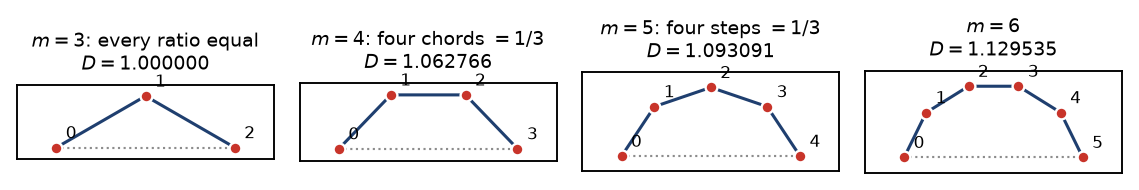
\includegraphics[width=0.95\textwidth]{small-m-optima.png}
  \caption{The optimal configurations at $m=3,4,5,6$, endpoint-gauged, with the chord dotted and the
  nodes numbered. $m=3$: all three ratios equal $2^{-\alp}$, i.e.\ an isosceles triangle with sides
  $1,2^{-\alp},2^{-\alp}$; $D=1$ exactly. $m=4$: four chords exactly $c=3^{-\alp}$ (the three
  steps and the end-to-end chord) and two chords $\sqrt{c(1+c)}/\sqrt3$. $m=5$: four steps exactly
  $1/3$ and the three chord-of-two steps equal. $m=6$: no such rigid structure, but the same
  pattern of two families of equal chords. The shapes get progressively less triangular --- a single
  corner, an $M$, an arch --- and $m=6$ still lies entirely on one side of its chord; the two-lobed
  $S$ of Figure~\ref{fig:ladder} appears only at the larger $m$.}
  \label{fig:smallm}
\end{figure}

Below, the $m=4$ case in full, since it is the one with a closed form.

\begin{proposition}\label{prop:m4}
Let $c=3^{-\alp}=0.4186878435451467$ and $K=\sqrt{(1+c)/(3c)}$. Then
\[
  K-2\times10^{-12}\ \le\ D_4\ \le\ K,\qquad K=1.062765923076354\ldots
\]
The upper bound is attained by the four points
\[
  v_0=0,\quad v_1=a+bi,\quad v_2=1-a+bi,\quad v_3=1,
  \qquad a=\frac{1-c}{2},\quad b=\sqrt{c^2-a^2},
\]
with $b=0.301361169565585\ldots$,
for which $r_{01}=r_{12}=r_{23}=r_{03}=c$ and $r_{02}=r_{13}=\sqrt{c(1+c)}/\sqrt3$. Hence
$D_\infty\ge1.0627659230747$.
\end{proposition}

\begin{proof}[Proof (computer-assisted)]
After the similarity gauge $v_0=0$, $v_3=1$ the problem is four-dimensional, in $(v_1,v_2)\in\mathbb{C}^2$,
and the six ratios are $r_{01}=|v_1|$, $r_{12}=|v_1-v_2|$, $r_{23}=|v_2-1|$, $r_{02}=|v_2|/\sqrt3$,
$r_{13}=|v_1-1|/\sqrt3$, $r_{03}=3^{-\alp}$, since $2^{\alp}=\sqrt3$ and $4^{\alp}=3$.

\emph{Upper bound.} For the displayed configuration $b^2=c^2-a^2$ gives $|v_1|=c$,
$v_2-v_1=1-2a=c$, $|v_2-1|=|a-bi|=c$ and, because $(1-a)^2+b^2=\tfrac14[(1+c)^2-(1-c)^2]+c^2=c(1+c)$,
also $|v_2|=|v_1-1|=\sqrt{c(1+c)}$. So four ratios equal $c$ and two equal $\sqrt{c(1+c)}/\sqrt3$,
and the quotient is $K$.

\emph{Lower bound.} If $D\le K$ then every ratio lies in $[c/K,Kc]$, which confines $(v_1,v_2)$ to the box
$\operatorname{Re}v_1\in[0.2293,0.4450]$, $\operatorname{Im}v_1\in[-0.4450,0.4450]$,
$\operatorname{Re}v_2\in[0.5550,0.7707]$, $\operatorname{Im}v_2\in[-0.4450,0.4450]$; outside it
$D>K$. On a box, rectangle arithmetic encloses each $r_{ij}$ in
$[\underline r_{ij},\overline r_{ij}]$ with outward rounding, and since $D\ge r_i/r_j$ pairwise,
$\max_{i\ne j}\underline r_i/\overline r_j$ is a lower bound for $D$ on the whole box. Discarding
boxes whose bound exceeds $K-10^{-12}$ and bisecting the rest along the widest coordinate leaves
$54\,163$ boxes in $0.07$ seconds, none surviving, which proves $D_4\ge K-1.7\times10^{-12}$
(\texttt{scripts/certify\_m4.py}). Four numbers to check independently: the interval bound was
tested against $16\,000$ sample points in $400$ random boxes, and $2\times10^5$ random
configurations produced none with $D\le K$ outside the a priori box.
\end{proof}

The minimiser is the symmetric bent chain $v_2=1-\overline{v_1}$, with four tight minimum pairs and
two tight maximum pairs; the certificate pins its position as well as the value, since every box
more than $10^{-12}$ away from it is discarded. The $m=5$ optimum has an equally rigid shape: four
consecutive chords exactly $1/3$ and the three chord-of-two steps equal, which is why the window
there closes to $10^{-6}$ with eighty boxes. What stops the method is dimension, not difficulty:
$m=7$ would need ten coordinates and the first-order bound is too weak to close.

\paragraph{Two macro-shapes, kept apart.} The searches return two families that do not mix. In the
first the gauged curve crosses its chord and carries one lobe on each side of it --- the S-shaped
branch of Figure~\ref{fig:ladder}. In the second it stays on one side, a single arch with a fractal
top, and its levels are compatible with one another across $m$ (Figure~\ref{fig:arc}). Both refine
coherently, so both are candidates for a limiting curve, and neither is selected here; what is
clear is that a ladder mixing them is not a sequence. Table~\ref{tab:ladder} therefore lists both,
and the rungs are quoted per branch.

\paragraph{The $m=200$ rung.} It used to be the arc, $1.5031685289$. An S-branch local minimum
exists at $m=200$: started from the $m=100$ S configuration with midpoints inserted and a kick, the
exact-minimax SLP converges in three rounds to
\[
  D_{200}=1.4908552600,
\]
with a multiplier certificate (48 tight maximum and 346 tight minimum pairs; the neighbouring
rounds give $1.4908867897$ and $1.4908781151$, so the value is stable at the fifth digit). That is
$0.82\%$ below the arc and $3.80\%$ above the $m=100$ value, so the ladder stays monotone, and it
is the entry in Table~\ref{tab:ladder} and the panel in Figure~\ref{fig:ladder}.

\begin{table}[t]
\centering
\small
\begin{tabular}{rrllrl}
\toprule
 & \multicolumn{3}{c}{S branch} & \multicolumn{2}{c}{one-sided arc branch}\\
\cmidrule(lr){2-4}\cmidrule(lr){5-6}
$m$ & best known $D_m$ & file & status & best known $D$ & status\\
\midrule
$40$   & $1.3523099782$ & \texttt{s\_m40.npy}          & stationary            & $1.3692601379$ & certified\\
$100$  & $1.4362283999$ & \texttt{s\_m100.npy}         & stationary            & $1.4475037000$ & certified\\
$200$  & $1.4908552600$ & \texttt{s\_m200.npy}         & first-order certified & $1.5031685289$ & stationary\\
$400$  & $1.5417920000$ & \texttt{s\_m400.npy}         & first-order certified & $1.5487020131$ & certified\\
$800$  & $1.5900261898$ & \texttt{s\_m800.npy}         & first-order certified & $1.5939535359$ & not certified\\
$1600$ & $1.6355308997$ & \texttt{s\_m1600.npy}        & stationary            & $1.6315839649$ & not certified\\
\bottomrule
\end{tabular}
\caption{Best known $m$-point distortions, in the two macro-shapes that the searches keep returning:
the S-shaped branch, whose gauged curve has one lobe on each side of its chord, and the one-sided
arc branch, which stays on one side of it (Figure~\ref{fig:arc}). ``First-order certified'' (or
``certified'') means a multiplier vector on the tight maximum and minimum pairs exists, so no
descent direction does; it says nothing about other basins, and no $D_m$ here is proved optimal.
The two branches are listed separately because mixing them makes the ladder jump: the entry at
$m=200$ used to be the arc, which is $0.8\%$ above the S value now recorded there.}
\label{tab:ladder}
\end{table}


\subsection*{Parts of the curve that repeat}\label{sec:blocks}

The numerical optima are not self-similar in shape. But parts of one curve do resemble other parts
of it, sometimes at another scale, and that is what Figure~\ref{fig:similar} shows. The search asks,
for two index intervals $I=[a,a+L]$ and $J=[c,c+K]$, whether
\[
  V(c+Kt)\ \approx\ s\,V(a+Lt)+d,\qquad t\in[0,1],
\]
with $s,d\in\mathbb{C}$ --- a similarity carrying the block onto the arc, the parameter taken
affinely --- and scores it scale free: both blocks are centred and divided by their own diameter and
only a rotation is fitted, so a residual of $0.10$ means the shapes agree to $10\%$ of the diameter,
with the size ratio $|s|$ reported separately. (Scoring the raw least-squares fit instead lets a
small arc match almost anything, because its errors are never amplified; a first version of this
search did exactly that and produced spurious $3\%$ hits.)

\begin{figure}[t]
  \centering
  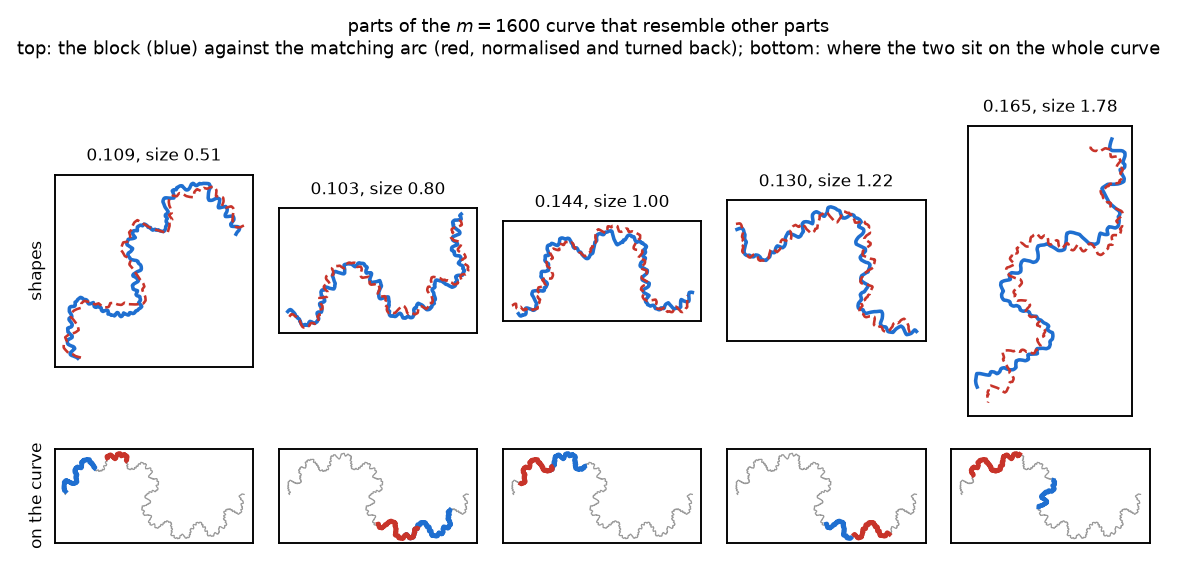
\includegraphics[width=0.95\textwidth]{block-similarity.png}
  \caption{The best matches between different parts of the $m=1600$ configuration, one per bin of
  size ratio. Top: the block in blue against the matching arc in red, dashed after normalising and
  turning it back; residuals $0.10$--$0.17$ of the block diameter at size ratios $0.51$, $0.80$,
  $1.00$, $1.22$, $1.78$, with rotations up to $136^\circ$. Bottom: where those two pieces sit on
  the whole curve, which is drawn thin and grey.}
  \label{fig:similar}
\end{figure}

The systematic search (\texttt{scripts/search\_overlaps.py}) comes with the control that matters.
Against the \emph{shuffled-turn} surrogates, which have the same step lengths and the same multiset
of turning angles in random order, and so the same roughness statistics but no sequence: at
$m=1600$ the real curve reaches residual $0.098$ with $34$ pairs below $0.12$ and $261$ below
$0.15$, while the surrogates reach $0.164$ and $0.169$ with nothing below $0.12$. So the order of
the steps matters, and these are not generic features of a rough curve. Two further checks are in the
earlier reports: at $m=800$ the best residual is $0.114$ ($0.158$ on the coarse shape), and an
alignment found at $m=800$ survives at $m=1600$ at doubled indices in the zeroth percentile against
the controls, so it is a property of the sequence and not a finite-size accident.

\paragraph{What a block sees of the distortion.} A different and sharper question about blocks has a
clean answer. For a self-similar arc a block that is a copy of the whole carries a copy of the whole
$r$-field, so it must return the same distortion, and it does: at level 6 the four level-1 pieces of
the Koch polygon each give $D=2.096805160875$ (deviation $2\times10^{-15}$), and the two pieces of
the two-piece arc at level 10 give $3.7\times10^{-15}$ and $2.2\times10^{-16}$. A shallower block is
a copy of a shallower \emph{truncation}, so it returns that truncation's value --- the level-3 blocks
of the Koch polygon give $2.089552$, the level-3 distortion, not an error.

For the numerical ladder this is a property rather than a theorem, and it holds. An exhaustive check
of all $205\,120$ contiguous blocks with gap at least $160$ of the stored $m=800$ configuration found
every one reproducing $D$ to $2.9\times10^{-6}$ relative, half of them to $10^{-9}$. On the polished
$m=800$ configuration it is much tighter (Figure~\ref{fig:blocks}): every block of length at least
$160$ reproduces $D$ to $1.2\times10^{-13}$, and the \emph{median} block is that accurate already at
length $40$ --- though the worst block of length $40$ is off by $9\%$, so not every block is
representative.

\begin{figure}[t]
  \centering
  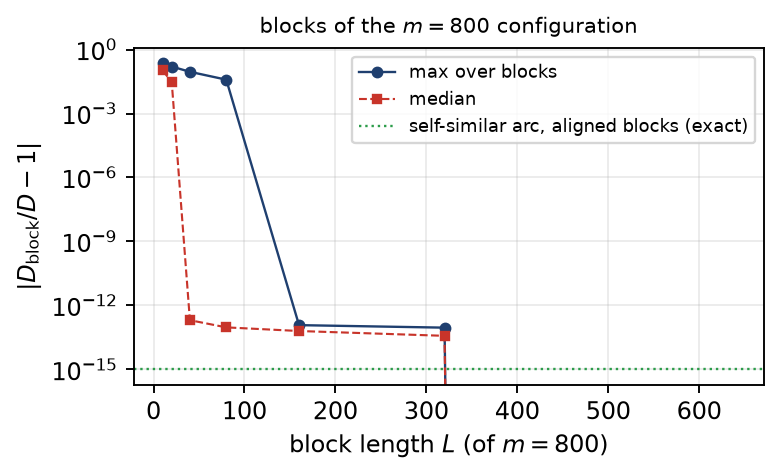
\includegraphics[width=0.68\textwidth]{block-comparison.png}
  \caption{Relative deviation of the restricted distortion $D_{\rm block}$ from the whole $D$,
  over all contiguous blocks of the $m=800$ configuration, against block length: the maximum over
  blocks and the median. The dotted line is the level a self-similar arc attains exactly at its
  substitution scales.}
  \label{fig:blocks}
\end{figure}

This is the combination to keep in mind: distant parts of the curve do \emph{not} agree in shape
($10\%$ residuals), but \emph{every} long block has the distortion of the whole ($10^{-13}$). The
numerical optima are locally self-similar in distortion without being self-similar in shape, which
is what one expects of the limiting object and is the strongest evidence in hand that it is not an
exactly self-similar curve.

\begin{figure}[t]
  \centering
  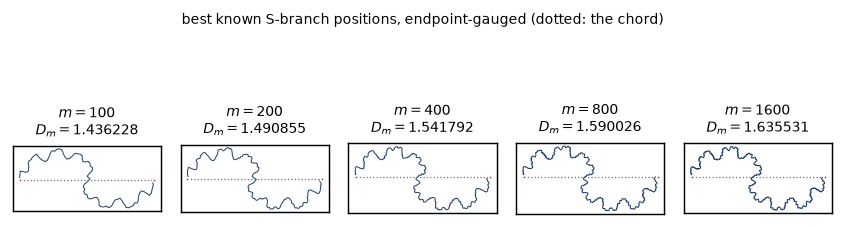
\includegraphics[width=\textwidth]{ladder-m.png}
  \caption{The S-branch configurations of Table~\ref{tab:ladder}, endpoint-gauged. From $m=100$
  upward they are visibly the same S-shaped profile with progressively finer microstructure; this
  is the sequence whose limit one wants to describe. The $m=200$ panel is the one found for
  \S\ref{sec:ladder}; the stored configuration it replaces had no lobe on the lower side at all.}
  \label{fig:ladder}
\end{figure}


\begin{figure}[t]
  \centering
  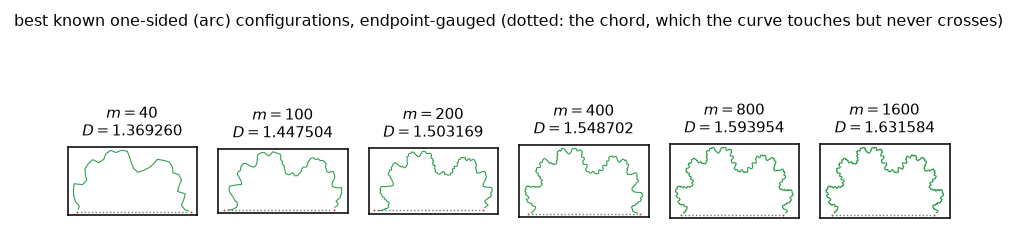
\includegraphics[width=\textwidth]{arc-m.png}
  \caption{The other branch: the best known one-sided (arc) configurations, endpoint-gauged. Here
  the gauged curve stays on one side of its chord --- one arch, no inflection --- and the family
  refines coherently with $m$ just as the S branch does. Its values are above the S branch from
  $m=40$ to $m=800$, by $1.25\%$, $0.79\%$, $0.83\%$, $0.45\%$ and $0.25\%$, and below it at
  $m=1600$ by $0.24\%$; the $m=1600$ pair is not certified, so that last ordering is provisional.
  Nothing here selects a branch: the two are recorded because a numerical ladder that mixes them
  is not a sequence.}
  \label{fig:arc}
\end{figure}

\begin{figure}[t]
  \centering
  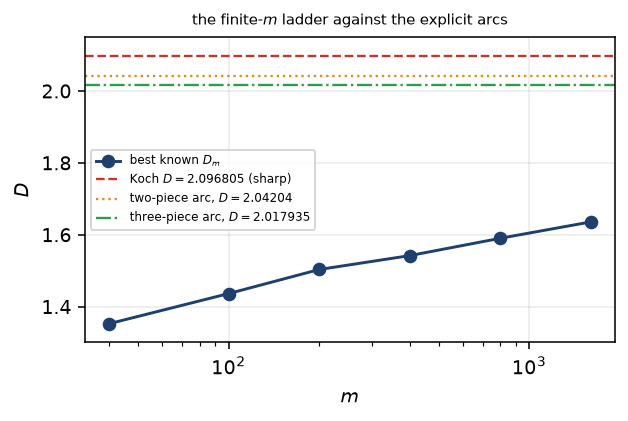
\includegraphics[width=\textwidth]{ladder-D.png}
  \caption{Left: the ladder against the explicit arcs --- $D_m$ still climbing ($1.35\to1.64$)
  while the best explicit curves sit at $2.02$--$2.04$; the vertical gap of about $0.4$ is the
  open problem. The dotted purple line is the certified lower bound
  $D_\infty\ge1.1195$ of \S\ref{sec:m4}, the red the proved upper bound: the problem
  lives in the strip between them, and the ladder shows that neither end is close. The bar on each
  point reaches the best value known in the \emph{other} branch at the same $m$ (the open squares),
  which is the only measured estimate of how far the point could move without leaving the search: it is $1.25\%$ of $D_m$ at $m=40$ and falls to $0.24\%$ at
  $m=1600$, where the arc is the better of the two. Right: that gap as a percentage. A branch
  crossing at $m=1600$ is not evidence that either branch is optimal --- only that the two are
  converging, so that the value of $D_\infty$ is pinned to within a per-cent by $m=1600$,
  whichever branch is used.}
  \label{fig:gap}
\end{figure}

\section{The gap, and what would close it}

Figure~\ref{fig:gap} is the whole point of this note. The ladder approaches $D_\infty$
\emph{from below} --- $D_m\le D_\infty$ --- so the numbers $1.3523,\dots,1.6355$ approximate lower
bounds for $D_\infty$, from below and from above at once: from below because $D_m$ is one, from
above because what we can compute at each $m$ is a minimising configuration, hence an upper bound
for $D_m$ and not a lower one. Only $D_4$ is certified. Across the gap stand the explicit curves,
which are genuine upper bounds: $2.0179$ measured, $2.0968$ proved. Nothing in hand says which side is close to
$D_\infty$.

\begin{enumerate}[label=(\alph*)]
\item \textbf{A certified arc below Koch.} The three-piece construction is explicit enough to be a
  theorem candidate: closed-form parameters, closure exact in $\R$, no optimisation. What is
  missing is a proved bound on the cross-piece pairs, i.e.\ a two-sided version of \eqref{eq:koch}
  for this map system, presumably by the same dyadic-parameter reduction used for Koch but with
  three addresses instead of four. This seems the most tractable genuinely new result in reach.
\item \textbf{Can an explicit arc reach the ladder?} If $D_\infty\approx1.6$--$1.7$ the existing
  constructions are far from optimal and a different idea is needed. The data suggest the optima
  are \emph{not} self-similar in the strict sense: their own sub-arcs are not copies, and the
  exact self-similar candidates that were tried all sit above $2.0$.
\item \textbf{Is the infimum attained?} By the compactness above, a limit of near-optimal
  configurations is optimal; what is unclear is whether the limit is unique, and the numerical
  ladder shows many distinct stationary configurations within a fraction of a percent
  (31 at $m=40$, 40 at $m=100$), so uniqueness of the \emph{selected} branch is not to be expected
  without a selection rule.

\item \textbf{The critical exponent.} The whole set-up makes sense for any $\alp\in(0,1)$, and the
  compactness argument gives $D_m(\alp)\to D^{(\alp)}_\infty$ for each. If a finite-distortion arc
  exists then its image has Hausdorff dimension $1/\alp$, so for $\alp<\tfrac12$ no such arc can
  exist: the Assouad dimension of $([0,1],|\cdot|^{\alp})$ is $1/\alp>2$, a bi-Lipschitz invariant,
  and a subset of the plane has Assouad dimension at most $2$. For $\alp>\tfrac12$ such arcs do
  exist, and not only for our exponent: Herron--Meyer (Rev.\ Mat.\ Iberoam.\ \textbf{28} (2012)
  603--630) prove that a metric quasicircle of Assouad dimension below $2$ is bi-Lipschitz
  equivalent to a planar one, and record that the same proofs cover bounded turning Jordan arcs
  and metric quasi-arcs. Our $\alp=\log3/\log4$ is in this range, and the Koch arc is the explicit
  witness. That leaves $\alp=\tfrac12$ exactly: is there an
  injective $\gamma\colon[0,1]\to\R^2$ with $|\gamma(x)-\gamma(y)|\asymp|x-y|^{1/2}$? We do not
  know, and we flag it as open rather than assert it. Equivalently, is $\sup_mD_m(\tfrac12)$
  finite? A first ladder at that exponent reads $D_m=1.1688$, $1.4323$, $1.7987$, $2.3386$,
  $3.4349$, $4.6863$ at $m=4,6,8,16,32,48,64$ -- rising by about $1.3$ per doubling, against
  $1.44\to1.64$ over a factor $16$ at $\alp=\log3/\log4$. That is what non-existence looks like,
  but it proves nothing, and the upper rungs are the least converged
  (\texttt{results/ladder-half.md}). The natural candidate, a self-similar arc with four maps of
  ratio $\tfrac12$ (the dimension-$2$ analogue of Koch), runs into the fact that the standard such
  curves are space-filling and therefore not injective, while the injective curves of Hausdorff
  dimension $2$ (Osgood's) are not known to admit a bi-Hölder parametrisation with exponent
  $\tfrac12$.

\item \textbf{Structure of the ladder.} The configurations' self-overlaps, their near-ties and the
  shape of the multiplier measures are the natural diagnostics; a companion note records what the
  overlap search says (many approximate self-similarities, thinning as $m$ grows).
\end{enumerate}

\section*{What is proved here, and what is not}

\begin{itemize}
\item Proved (elsewhere, in the companion note): \eqref{eq:koch} with both constants sharp; hence
  $D_\infty\le2.0968$.
\item Proved here, and elementary: $D(\gamma)>1$ for every injective arc, so $D_\infty>1$
  (\S\ref{sec:prior}, Cayley--Menger); and $\rho\le6$, i.e. \eqref{eq:crude}, which bounds the upper
  constant alone.
\item Proved here, computer-assisted: the windows of \S\ref{sec:m4} for $m=4,5,6$; in particular
  $D_4=1.062765923076\ldots$ (Proposition~\ref{prop:m4}) and $D_\infty\ge1.1195$.
\item Measured, not proved: $D=2.04204$ and $D=2.017935389$ for the two explicit arcs; every entry
  of Table~\ref{tab:ladder}, in both branches; the monotone ladders
  $1.3523\le\cdots\le1.6355$ (S) and $1.3693\le\cdots\le1.6316$ (arc).
\item Not known: any lower bound for $D_\infty$ beyond $1.1195$ (that is, any $D_m$ with $m\ge7$,
  or a tighter window at $m=6$);
  whether either explicit arc is optimal; which
  branch, if either, converges to the limit; whether $D_m$ converges rapidly enough to be
  extrapolated.
\end{itemize}

\appendix
\section*{Reproduction}
\begin{sloppypar}
\begin{itemize}
\item \texttt{scripts/explicit\_curves.py} builds both arcs from the formulas above and prints
  the level-$K$ ratios. The script
  \texttt{scripts/plot\_explicit\_and\_ladder.py} draws
  Figures~\ref{fig:curves}, \ref{fig:ladder}, \ref{fig:arc} and \ref{fig:gap}.
\item \texttt{scripts/plot\_construction\_stages.py} draws Figure~\ref{fig:stages}; it checks its
  own vertices against \texttt{explicit\_curves.py} before plotting.
\item All configuration data are in \texttt{data/}: \texttt{s\_m40.npy} to \texttt{s\_m1600.npy}
  (the S branch) and \texttt{arc40.npy} to \texttt{arc1600.npy} (the one-sided branch), one complex
  array of node positions each, endpoint-gauged; \texttt{m5\_best.npy} and \texttt{m6\_best.npy} are
  the configurations of Figure~\ref{fig:smallm}. The S-branch rows of Table~\ref{tab:ladder} are the
  \texttt{s\_m*} files;
  \texttt{scripts/optimise\_m400.py} produced the certified rows, including the new $m=200$ one
  (\texttt{--m 200 --start} a kicked upsampling of the $m=100$ configuration).
\item The last-named script draws Figures~\ref{fig:arc} and~\ref{fig:gap} from the
  \texttt{arc*.npy} and \texttt{s\_m*.npy} files in \texttt{data/}.
\item \texttt{scripts/certify\_mm.py} is the certificate of \S\ref{sec:m4} for any $m$; e.g.
  \texttt{--m 5 --eps 1e-6}, \texttt{--m 6 --eps 1e-2 --Dbar 1.129534712}. It prints the certified
  window; $m=4$ with \texttt{--m 4 --eps 1e-12} reproduces \texttt{results/m4-global.json}. \texttt{scripts/ladder\_half.py}
  is the $\alp=\tfrac12$ ladder of \S\ref{sec:prior} (results in \texttt{results/ladder-half.json}).
\item \texttt{scripts/restart\_study.py} re-runs a cheap optimisation from perturbed and resampled
  starts at each rung and records the values in \texttt{results/restart-study.json}. With the cheap
  budget it lands $0.1$--$1\%$ above the polished values at $m\ge200$, so it measures how much the
  answer depends on where the search starts rather than where the minimum is; together with the
  branch gaps it is what the bars of Figure~\ref{fig:gap} show.
\end{itemize}
\end{sloppypar}

\end{document}
